\newcommand{\bankdistance}{4}
\tikzstyle{bank}=[
  draw,
  minimum width=1.5cm,
  minimum height=1cm,
  font=\huge
]
\tikzstyle{op}=[
  -latex,
  ultra thick
]

\newcommand{\drawbanks}[6]{{
  \newcommand{\banka}{#1}
  \newcommand{\bankb}{#2}
  \newcommand{\bankaa}{#3}
  \newcommand{\bankbb}{#4}
  \newcommand{\bankaaa}{#5}
  \newcommand{\bankbbb}{#6}

  \node[bank, label=above:{Replica $A$}] (a1) at (0,              0) {\banka};
  \node[bank                           ] (a2) at (0,             -3) {\bankaa};
  \node[bank                           ] (a3) at (0,             -6) {\bankaaa};
  \node[bank, label=above:{Replica $B$}] (b1) at (\bankdistance,  0) {\bankb};
  \node[bank                           ] (b2) at (\bankdistance, -3) {\bankbb};
  \node[bank                           ] (b3) at (\bankdistance, -6) {\bankbbb};

  \draw[op] (a1) -- (a2);
  \draw[op] (a2) -- (a3);
  \draw[op] (b1) -- (b2);
  \draw[op] (b2) -- (b3);
}}

\newcommand{\zigzag}[2]{{
  \newcommand{\banka}{#1}
  \newcommand{\bankb}{#2}

  \draw[red, op] ($(\banka) + (0, -0.7)$) -- ($(\bankb) + (0, -1.0)$);
  \draw[red, op] ($(\bankb) + (0, -1.0)$) -- ($(\banka) + (0, -1.3)$);
  \draw[red, op] ($(\banka) + (0, -1.3)$) -- ($(\bankb) + (0, -1.6)$);
  \draw[red, op] ($(\bankb) + (0, -1.6)$) -- ($(\banka) + (0, -1.9)$);
}}

\begin{frame}{Replicated Bank Account}
  \begin{center}
    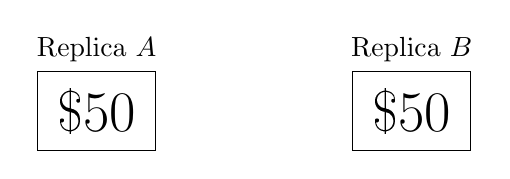
\begin{tikzpicture}
      \node[bank, label=above:{Replica $A$}] (a1) at (0, 0) {\$50};
      \node[bank, label=above:{Replica $B$}] (b1) at (\bankdistance, 0) {\$50};
    \end{tikzpicture}
  \end{center}

  \note{%
    We'll begin with an example.

    Let's say we want to replicate the database shown here. This database is
    the world's simplest database. It contains only a single number, which
    represents my bank account balance. We decide to replicate this database
    across two machines, replica A and replica B.

    Users can issue transactions to the database, and every transacation is
    either a deposit or a withdrawal. And, I have one critical invariant that I
    want to maintain over my database. And that invariant is that my bank
    account balance should never be negative. My balance must be non-negative at all times.
  }
\end{frame}

\begin{frame}{Coordinating}
  \begin{center}
    \begin{tikzpicture}
      \drawbanks{\$50}{\$50}
                {\$60}{\$60}
                {\$80}{\$80}

      \draw[op] ($(a1) + (-2, 0)$) -- (a1) node[midway, above] {$+\$10$};
      \draw[op] ($(b1) + (+2, 0)$) -- (b1) node[midway, above] {$+\$20$};
      \draw[op] (a2) -- ($(a2) + (-2, 0)$) node[midway, above] {OK};
      \draw[op] (b3) -- ($(b3) + (+2, 0)$) node[midway, above] {OK};

      \zigzag{a1}{b1}
      \zigzag{a2}{b2}
    \end{tikzpicture}
  \end{center}

  \note{%
    One way to replicate our database is by using coordination to implement
    strong consistency. For example, imagine a user issues a deposit of 10
    dollars to replica A, and simultaneously, a user issues a deposit of 20
    dollars to replica B. The two replicas can coordinate, for example by
    running Paxos, and agree on a single total order in which to execute the
    two transactions. Here, the replicas agree to deposit 10 dollars and then
    deposit 20 dollars. Both transactions succeed, and the replicas send back OK
    messages to the clients letting them know everything went smoothly.
  }
\end{frame}

\begin{frame}{Coordinating}
  \begin{center}
    \begin{tikzpicture}
      \drawbanks{\$50}{\$50}
                {\$20}{\$20}
                {\$20}{\$20}

      \draw[op] ($(a1) + (-2, 0)$) -- (a1) node[midway, above] {$-\$30$};
      \draw[op] ($(b1) + (+2, 0)$) -- (b1) node[midway, above] {$-\$40$};
      \draw[op] (a2) -- ($(a2) + (-2, 0)$) node[midway, above] {OK};
      \draw[op] (b3) -- ($(b3) + (+2, 0)$) node[midway, above] {NO};

      \zigzag{a1}{b1}
      \zigzag{a2}{b2}
    \end{tikzpicture}
  \end{center}

  \note{%
    Now, assume two clients issue concurrent withdrawal transactions of 30
    dollars and 40 dollars. Again, the two replicas coordinate and agree to
    execute the withdrawal of 30 dollars and then the withdrawal of 40 dollars.

    The withdrawal of 30 dollars executes fine, brining my bank account balance
    to 20 dollars, but the withdrawal of 40 dollars fails because I only have
    20 dollars left. So replica A sends back an OK message to the client, but
    replica B sends back a NO message letting the client know the transaction
    failed. And while the transaction failed, you'll note that we never
    violated our application invariant.
  }
\end{frame}

\begin{frame}{Avoiding Coordination}
  \begin{center}
    \begin{tikzpicture}
      \drawbanks{\$50}{\$50}
                {\$60}{\$70}
                {\$80}{\$80}

      \draw[op] ($(a1) + (-2, 0)$) -- (a1) node[midway, above] {$+\$10$};
      \draw[op] ($(b1) + (+2, 0)$) -- (b1) node[midway, above] {$+\$20$};
      \draw[op] (a2) -- ($(a2) + (-2, 0)$) node[midway, above] {OK};
      \draw[op] (b2) -- ($(b2) + (+2, 0)$) node[midway, above] {OK};

      \draw[dashed, op] (a2) -- (b3) node[near start, sloped, above] {$+\$10$};
      \draw[dashed, op] (b2) -- (a3) node[near start, sloped, above] {$+\$20$};
    \end{tikzpicture}
  \end{center}

  \note{%
    Alternatively, instead of implementing our bank with strong consistency, we
    could implement it with weak consistency and avoid coordination altogether.

    Now, when two clients issue concurrent deposit transactions, the two
    replicas execute the transactions immediately without consulting one
    another. And every once in a while, the two replicas communicate and fill
    each other in on the transactions they missed.

    Here, for example, replica A lets replica B know to deposit 10 dollars and
    replica B lets replica A know to deposit 20 dollars. Notice that even
    though we didn't perform any coordination, the two replicas never violate
    my critical invariant of a non-negative balance.
  }
\end{frame}

\begin{frame}{Avoiding Coordination}
  \begin{center}
    \begin{tikzpicture}
      \drawbanks{\$50}{\$50}
                {\$20}{\$10}
                {-\$20}{-\$20}

      \draw[op] ($(a1) + (-2, 0)$) -- (a1) node[midway, above] {$-\$30$};
      \draw[op] ($(b1) + (+2, 0)$) -- (b1) node[midway, above] {$-\$40$};
      \draw[op] (a2) -- ($(a2) + (-2, 0)$) node[midway, above] {OK};
      \draw[op] (b2) -- ($(b2) + (+2, 0)$) node[midway, above] {OK};

      \draw[dashed, op] (a2) -- (b3) node[near start, sloped, above] {$-\$30$};
      \draw[dashed, op] (b2) -- (a3) node[near start, sloped, above] {$-\$40$};
    \end{tikzpicture}
  \end{center}

  \note{%
    However, let's look what happens when two clients issue concurrent
    withdrawals. Both withdrawals are executed locally and both succeed.
    However, when the two replicas exchange transactions with one another, they
    both enter an invariant violating state of negative twenty dollars!
  }
\end{frame}

\begin{frame}
  \begin{center}
    \Huge
    Deposits don't require coordination to maintain invariants, but withdrawals
    do.
  \end{center}

  \note{%
    We can learn a lot from these examples.

    First, if we implement our bank with strong consistency, we never violate
    our invariant.

    Second, we can implement deposit transactions without any coordination and
    we're still guaranteed to never violate the invariant.

    Third, withdrawal transactions, unlike deposit transactions, do require
    coordination to avoid violating the invariant.

    At a very high level, invariant confluence tries to capture exactly which
    transactions require coordination to maintain invariants and which do not.
    In this example, deposit transactions are invariant confluent and thus do
    not require coordination while withdrawal transactions are not invariant
    confluent and thus do require coordination.
  }
\end{frame}
